		\subsubsection{Electrical Connection Mechanism}

		The core of this project is the hot swapping device.  The electrical connection that allows the transfer of power, audio, and control signals between the a universal adapter plate and the module containing the hot swapping device is vital.  Though a number of guitar pedals offer processing of stereo signals, most are fully monophonic, requiring only one input and output connection.  In addition, because almost every pedal uses a single supply (non-bipolar) voltage, the simplest scheme for connecting a plate to its receiver requires only four connections: Power, Ground, Input (Send), and Output (Return). This means that it is feasible to transfer the signal directly with individual physical connections, rather than some serial data protocol such as I$^2$S, which might be used if there were many inputs and outputs.  The use of ”hard-wire” connections also keeps the signal ”pure” by eliminating any unnecessary processing, which is an important consideration for marketing purposes.  

		Making a consistent electric connection between the plate and receiver calls for some sort of spring loaded connector.  They should be able to easily mate or break, but must maintain good contact when connected.  They should not require the two surfaces to be exactly aligned, and they should require only the single part to operate (instead of a matching male and female connector) for cost purposes.  Figure \ref{fig:springloaded} shows some examples of spring loaded connectors.  On the left are connectors typically used to connect boards together within a product. This class of spring connector is good for high pin count connections because of the large number of pins in a single unit, which are easy to manufacture cheaply. For example, the 00-9258 type connector from AVX Corp costs \$0.77 for 8 electrodes from Digikey. However, because these connectors are usually made for one time use when permanently assembling a product, they are not designed for repeated use. For instance, the 00-9258 part is has a lifespan of just 50 cycles according to its datasheet, which is certainly insufficient for this application. For an order of magnitude estimate, each plate needs to be able to withstand 100 cycles per day for at least 1000 days (though the cycles/day is likely lower and the total days is likely higher). This gives a ballpark estimate of 100,000 cycles minimum.  Spring loaded pins like those to the right in Figure \ref{fig:springloaded} were the preferred type of connector.  This type of connector, sometimes known as a ”Pogo Pin,” includes a spring loaded plunger that sheaths into a sleeve. These can be sourced through Digikey from Mill-Max, an industry standard manufacturer of milled connectors. They have excellent electrical and mechanical characteristics, including 20m\ohm contact resistance, minimum of 2 amp current rating, and a 1,000,000 cycle lifespan which makes them an excellent choice for this application.  The downside is in cost, as a single pin in the standard 0906 series costs \$0.44 each from Digikey, but the requirement for durability outweighs this drawback.

		\begin{figure}
			\centering
			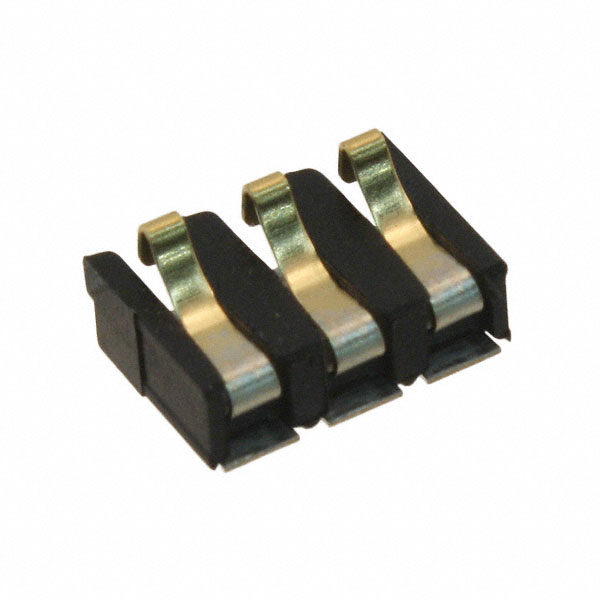
\includegraphics[width = 0.4\linewidth]{PR2Images/batteryconn}
			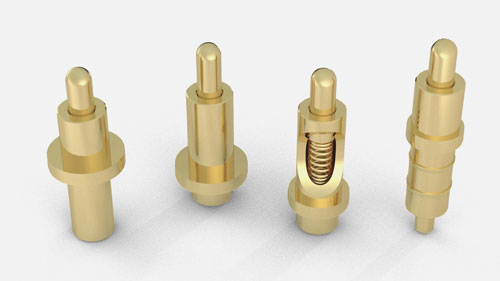
\includegraphics[width = 0.4\linewidth]{PR2Images/springpin.jpg}
			\caption{Examples of spring loaded connectors.  On the left is a battery type connector with leaf type springs.  On the right is a spring loaded pin type connector, often known as a "pogo pin".}
			\label{fig:springloaded}
		\end{figure}

		The 0906-1 model spring loaded pin was chosen because of its low cost relative to other series, and because it had a relatively short length (0.177") which reduces torques on the contact point between the pin and the circuit board due to any tangential force on the end of the pin, which is held in place only with solder.  This serves to increase durability; the through-hole mounting style was chosen over surface mount for the same reason.

		Initially, the design featured pogo pins of varying heights to enable a mate-first, break-last connection.  This was done with the intention of ensuring that the audio signals are never connected without the power also being connected, to avoid unnecessary pops and transients in the audio signal.  However, testing of a prototype hot swapping connector showed that the weight of the plate and pedal alone was not enough to activate both the taller and shorter pins, requiring additional force to make all connections.  Though this could have been fixed using a magnetic system to add the required force, a more sophisticated controlling mechanism (see below) was used to prevent the signal from being connected too soon, resulting in the same benefits as the varied height design without the issues with connection.

		Because most guitar effects pedals have only mono I/O and all of them support mono operation even if they do have stereo capability, the hot swapping device was designed to operate only in mono, although the design can easily be extended to stereo operation in the future.  This means that two pins are required for the audio signals, in addition to ground.  The power supply requires an additional power pin plus a second ground pin.

		\subsubsection{Pedal Power Selection}

		In order to maximize the compatibility metric, the solution should be able to supply the most commonly required voltage and current supplies.  Though 9VDC is the de facto standard voltage supply \cite{MyPedalData}, there are a number of effects that accept 12 or 18 VDC, which can allow their amplifiers to have a higher headroom.  There are some other less common power supplies, such as 24 VDC for some older Electro Harmonix products, or 9 VAC for pedals like the Line 6 DL4 \cite{Line6DL4manual}, but these are rarer, so the design focused on just the 9, 12, and 18 VDC supplies.  Users can select which power supply is used on each plate, and the desired power is automatically connected.

		In order to supply power to the plate, two schemes were considered.  The first was a parallel supply, where all three voltages are connected to the plate at once, and the user who sets up the plate for a particular pedal can choose which connector to attach the power connector to.  This would allow a single voltage regulator for each supply voltage to be used.  However, this could run into issues of current draw, where many pedals could potentially draw more current than the voltage regulator can handle.  In addition, this would mean long traces in the main board carrying this voltage, which might experience a voltage drop due to the resistance of these traces.  Figure \ref{fig:parallelpowerschematic} shows an implementation of such a scheme.

		\insertimage{0.5}{PR2Images/ParallelPowerSchematic.PNG}{Power supply implementation where all voltages are available at all times.}{fig:parallelpowerschematic}

		The other option was to use a single voltage regulator for each plate, with a controllable output.  This eliminates concern over voltage drops between different receivers, and allows each receiver to draw as much current as a single regulator can supply.  For more than two power outputs, this method saves pogo pins, as only two pins are needed to supply the power (in addition to ground), though it does require several pins to communicate which voltage is desired for the current plate.  Instead of multiple connectors to allow the user to select the power connection, this method would use some switch, such as a two position DIP switch, to allow the user to set a binary value which can be decoded on the receiving end into the proper signals needed to control the adjustable voltage regulator.  As the pogo pins are fairly expensive (about \$0.66 each), reducing the number of pins is a good way to save on cost.

		The LM317 is a canonical adjustable voltage regulator, with its level set via a voltage divider (see datasheet section 8.2 for a typical application and design requirements \cite{LM317datasheet}).  The LM317 takes an input voltage between 1.25 and 37 V, preferably with $V_I - V_O > $ 3 V.  The difference $V_{OUT} - V_{ADJUST}$ is then kept at 1.25 V with a feedback circuit.  As shown in Figure \ref{fig:LM317_typicalapp}, this 1.25 V reference and $R_1$ then set the current through variable resistor $R_2$ ($I_{Adj}$ is negligible) which controls the output.  The 240\ohm value for $R_1$ is a recommended value required to keep the output current high enough (over 3.5 mA) for a well regulated output.  The other diodes and capacitors are used to reduce ripple in the output.  Thus, $V_O$ can be given by

		\begin{align}
			V_O &= V_{REF}(1 + \frac{R_2}{R_1}) + I_{ADJ}R_2 \\
			&= 1.25 (1 + \frac{R_2}{240}) \quad \text{and} \\
			R_2 &= 240 \left( \frac{V_O}{1.25} - 1 \right) \\
			\label{eqn:LM317_R2}
		\end{align}

		However, a variable resistor for $R_2$ is not an easy method of setting the proper voltage for a user, because this would require individual tuning for each plate.  Instead, a set of switches is an easy mechanism for a user, who just needs to set the correct position of the switches.  A straightforward technique to use is switch in and out some additional resistors in parallel to a fixed $R_2$, as shown in Figure \ref{fig:adjustableregulatorschematic}.  Adding resistors in parallel reduces the effective resistance, reducing the output voltage, so the fixed $R_2$ should be calculated to set the maximum required output voltage, 18 VDC.  Using Equation \ref{eqn:LM317_R2} to calculate $R_2$ for an 18 V output gives $R_2 = 3.2 \text{\kohm}$. The current through $R_1$ and consequently $R_2$ is $i_{R_1} = 1.25/240 = 5.2$ mA.  

		\insertimage{0.8}{PR2Images/LM317_typicalapplication}{Typical Application of LM317, from datasheet.}{fig:LM317_typicalapp}

		\insertimage{0.8}{PR2Images/AdjustableRegulatorSchematic}{MOSFET controlled adjustable regulator, with 9, 12, and 18 VDC selectable output.}{fig:adjustableregulatorschematic}

		MOSFETs are a good choice for this switch application because of their relatively low on-resistance $R_{DSon}$.  The cheapest type of MOSFET available from Digikey was the NX7002AK type, a ubiquitous single N-channel device \cite{NX7002AKdatasheet}.  With a maximum $V_{DS}$ of 60 V, a maximum $I_D$ of 190 mA for $V_{GS} = 10$ V at $25^o$ C, and a typical $R_{DSon}$ of 3.7\ohm at $V_{GS}$ = 5V, this will work fine for this application, as would many standard MOSFETs.  In fact, because $R_{DSon}$ is on the order of Ohms while $R_2$ is on the order of \kohm, it can be neglected in the calculations for $R_3$ and $R_4$.

		For simplicity, assume the MOSFET gate signals will not be turned on together, and that Q3 is used for a 9 V output while Q4 is used for a 12 V output, as in the following truth table:

		\begin{center}
		\begin{tabular}{c c|c}
			Q3 & Q4 & Output Voltage (V) \\
			\hline
			0 & 0 & 18 \\
			0 & 1 & 12 \\
			1 & 0 & 9 \\
			1 & 1 & X
		\end{tabular}
		\end{center}

		Because the MOSFET's on resistance can be ignored, solving for the $R_3$ when $Q_3$ is turned on so $R_3$ and $R_2$ are connected in parallel to ground gives

		\begin{align}
			R_3 || R_2 &= R_1 \left( \frac{V_O}{1.25} - 1 \right) = 240 \left( \frac{9}{1.25} - 1 \right) = 1488 \\
			R_3 &= \frac{1}{\frac{1}{R_3 || R_2} - \frac{1}{R_2}} = \frac{1}{\frac{1}{1488} - \frac{1}{3200}} = 2.8 \text{\kohm}
		\end{align}

		Likewise, 

		\begin{align}
			R_4 || R_2 &= R_1 \left( \frac{V_O}{1.25} - 1 \right) = 240 \left( \frac{12}{1.25} - 1 \right) = 2064 \\
			R_4 &= \frac{1}{\frac{1}{R_4 || R_2} - \frac{1}{R_2}} = \frac{1}{\frac{1}{2064} - \frac{1}{3200}} = 5.8 \text{\kohm}
		\end{align}

		Compute the power dissipated across these resistors to determine their necessary ratings.

		\begin{center}
		\begin{tabular}{c c|c}
			R (\kohm) & V (V) & P (mW) \\
			\hline
			$R_1$ = 0.240 & 1.25 & 6.51 \\
			$R_2$ = 3.2 & 18 - 1.25 = 16.75 & 87.68 \\
			$R_3$ = 2.8 & 12 - 1.25 = 10.75 & 41.27 \\
			$R_4$ = 5.8 & 9 - 1.25 = 7.75 & 10.36
		\end{tabular}
		\end{center}

		Even with a 10\% safety margin, these resistors can all be 1/10 watt.

		\subsubsection{Hot Swap Event Detection}

		To perform the automatic bypassing feature, the receiving side of the hot swapping connector must detect whether or not a plate has been inserted. To do this, some of the same type of electrodes used to make connection between the plate and the receiver for signal and power where used as SPST switches.  When no plate is inserted, the switch is open, and when a plate is inserted, the switch closes. This can signal some logic circuitry to actuate the actual signal switching device.  To reduce transients that could result from suddenly connecting a plate and allowing the signal to flow before all of the necessary connections (Power, Ground, Input, and Output) are made, the receiver should wait to switch the relay from bypass to active until all of the pins have made their connections.

		Two of these switch pins were used.  Out of convenience and the ability to integrate Mill-Max's complementary pogo pin targets if necessary, the whole set of pins were arranged in a single row with 0.1" pitch.  The switch pins were placed on either end of this row.  Assuming a flat plate, this means that if both of the switch pins have made contact with the plate, then the rest of the pins must have also made contact.

		Electrically, these switch pins were each connected to an input of a microcontroller, with pull up resistors enabled.  When no plate is present, these GPIO are pulled high through these pull-ups.  On board the plates, the mating electrodes for the switch pins are both connected to the ground electrode, so when a plate is inserted into the hot swapping receiver, the switch pins are connected to ground and the microcontroller inputs are pulled down.  A logical AND on the debounced values of these switched is used by the microcontroller to determine if the plate has been inserted.

		The debounce routine used for these pins is performed in parallel on each of them.  It ensures that the value of the GPIO has remained constant for $20ms$ after it detects a change in the pin before the signal is asserted to the rest of the program.  The debouncing of the switch pins also allows the power and audio signal pins to connect before the audio signal is sent to the pedal.

		\subsubsection{Hot Swap Event Actuation}

		Once the microcontroller detects that a plate has been inserted or removed from the hot swapping receiver, it must initiate the actual signal switching.  The primary function of the hot swapping device is to automatically bypass any receivers that do not currently have a plate inserted, so the choice of switching element is a key part of the design. The basic choice here was between solid state analog switches or electromechanical relays. The major design considerations for this choice are the signal to noise ratio, and the frequency response of the switching element. 

		The initial value measured for the noise floor for an electric guitar was near $-90dBV$.  Guitar pickups convert the mechanical energy of the vibrating strings to electrical energy via a coil of wire. When the string vibrates in the magnetic field of a permanent magnet situated underneath, current is induced in the coil. In an ideal environment, there should be little source of self noise because of the passive simplicity of this device, so any noise in the guitar signal is a result of the environment. As such, the signal to noise ratio of a guitar can vary significantly based on the guitar’s environment. For example, guitar pickups are well known for their susceptibility to 60Hz line noise. Therefore, the measured 90dBV signal to noise ratio should be taken as a minimum value, with 100dBV or more preferable. While solid state switches are more size, cost, and power efficient than mechanical relays, they may not have adequate signal to noise specifications, as well as crosstalk between channels on the same chip. For example, the MT8808 Analog Switch Array lists no specification on the device’s signal to noise ratio, though it does boast a reasonable $-90dB$ crosstalk between any channels for a 10kHz input with a 600\ohm load. The feed-through when a channel is off is listed as $-95dB$ though, which is does not far exceed the minimum measured value for guitar signal to noise ratio, which could be an issue. On the other hand, relay bypassing utilizing mechanical switches has no issues with signal to noise ratio, which would make it suitable for use in this project.

		As a minimum, the system should accommodate signals across the full range of human hearing, which is typically noted as 20Hz - 20kHz. While this is the minimum acceptable range, there should also be allowance for lower and higher frequencies, which when used as input to a distortion effect can create inter-modulation distortion with frequencies in the audio range. Neither of these ranges will be an issue however. In the case that switching is accomplished with a solid state device, these are designed for frequency responses up to the tens of MHz range (the MT8808 has a 3dB frequency response of 45MHz), which is far greater than required. If mechanical relays are used, there will likewise be no issues with frequency response in the audio range.

		\insertimage{0.4}{PR2Images/GuitarPickupModel}{Model of guitar circuit.  These values are highly dependent on the particular pickups.  The potentiometer is either 250\kohm or 500\kohm.}{fig:guitarpickupmodel}

		These considerations suggest a preference for using mechanical relays despite their costs. An additional reason is some of the interactions between the circuits on the guitar and in the first engaged pedal. As mentioned above, the guitar pickup is made from a coil of wire, typically about 42 AWG with thousands of turns around a 6 inch or so circumference bobbin. This long thin wire produces a DC resistance on the order of 10\kohm, which itself is quite a high output impedance, and the inductance and some parasitic capacitances from within the pickup will result in a frequency dependent output impedance with the potential to interact with a connected circuit block with sufficiently low input impedance. In addition, the position of the guitar’s volume potentiometer can affect the output impedance (see Figure \ref{fig:guitarpickupmodel} for a model of a guitar pickup and volume control circuit). There are a number of guitar pedals known for their interaction with the guitar’s volume knob.  This does not follow the rule of thumb suggesting the input impedance should be an order of magnitude greater than the output impedance of the previous circuit stage, which means that there will be interactions between the guitar and this pedal.

		Whether or not these interactions are good or bad, they have an undeniable effect on the sound and feel of playing the guitar through this pedal. Inserting a buffer, including a solid state switch, between these circuit elements would destroy this interaction, and thus would prevent the solution from being an effect tool for comparing different pedals. Therefore, the signal path should pass through no buffers when all receivers are bypassed, and electromechanical relays should be used to perform the switching.

		To choose the relay, several criteria were considered, as listed in Table \ref{tab:relay_criteria}.  During the prototype design, the Kemet EA2-5SNJ was chosen as the best candidate.  The single coil latching Form-C DPDT relay had the best combination of the desired properties for the best price.  However, when it came time to build the full system with multiple modules in the spring, the EA2-5SNJ had become obsolete, and had to be replaced with the similar UD2-5SNU.

		\begin{table}
		\begin{center}
		\begin{tabular}{ |c p{3in} c| }
		\hline
		\multicolumn{3}{|c|}{\large Relay Selection Considerations \normalsize} \\
		\hline
		Criteria & Description & Desired Value\\ 
		 \hline
		Coil Voltage 	& The voltage required to activate the relay.  Higher voltages typically require less current because of higher coil resistances.  While it is beneficial to minimize relay coil current, it is often easier to use a lower coil voltage for easier interfacing with logic circuits or microcontrollers.  & 5V \\
		Switch Type 	& DPDT, SPDT, SPST, etc... a DPDT allows a single device to activate the bypassing for an entire hot swapping device.  & DPDT \\
		Actuation Type 	& Non-latching, Single Coil Latching, Double Coil Latching.  Non-latching is simplest but requires continuous current to keep relay in "set" state.  Both latching types require more complex control circuits & Latching \\
		Contact Type 	& Form A, B, C.  The first two relate only to SPST.  Form C indicates that a xPDT relay will break one connection before making the other, which is desired so two outputs are never connected together simultaneously. & Form C  \\
		Cost 			& This is self explanatory, but it is important to consider the total cost required to perform the desired action.  For instance, two SPDT relays would be required to do the same job as a single DPDT, so the SPDT relays would need to each be less than half the price of the DPDT to be preferred. & Minimum per pole \\
	   	\hline
		\end{tabular}
		\caption{Considerations used to select particular relay device.}
		\label{tab:relay_criteria}
		\end{center}
		\end{table}

		These relays use a single-coil latching actuation method, where the coil is s energized in one polarity to set the switch to one position, and is energized in the opposite polarity to set the switch to the other position. This calls for an H-bridge style driver.

		\insertimage{0.6}{PR2Images/DiscreteHBridge.png}{Discrete H Bridge implementation.  The inductor coil K1C load is the relay coil.}{fig:DiscreteHBridge}

		A standard discrete H bridge like the one shown in Figure \ref{fig:DiscreteHBridge} uses a quartet of transistors to power a load in either polarity or not at all.  When the two transistors in opposite corners (such as Q1 and Q4) are turned on at the same time, current flows through these transistors and the load, in this case the latching relay coil.  When it is time to set the relay's switch to the opposite position, the other two transistors are turned on instead and the load is energized with opposite polarity.  This implementation features garden-variety 3904/3906 type BJTs, which can supply plenty of current for the relay coil (just $5V/250\Omega = 20 mA$), though these many other transistors would work.  D1-D4 are flyback diodes for the inductive relay coil.  To provide a load current of 

		\begin{align}
			i_{load} &= \frac{5V - V_{CE_4} - V_{CE_1}}{250 \Omega} = 18.4 mA
		\end{align}

		the base current of the transistors is related to the collector current by

		\begin{align}
			I_B &= \frac{I_C}{\beta}
		\end{align}

		The 2N3904 has a $\beta$ between 100 and 300 for a 10 mA $I_C$, so assuming $\beta = 200$ gives a required base current of

		\begin{align}
			I_B &= \frac{18.4mA}{200} = 92 \mu A \quad \text{and} \\
			R_2 &= 4.3V/92\mu A = 43 k\Omega
		\end{align}

		For a 10\% tolerance, use a $39k\Omega$ to ensure the transistor is turned fully on.

		A major issue with the H-bridge design is that both sets of transistors can never be turned on at the same time.  This would create a low impedance path from power to ground, cause high currents and potential damage to the circuit.  Though more of an issue in PWM motor control, a common application of the H-bridge, this "shoot-through" can occur when one set of transistors is switched on just as the other set is switched off.  Special protection must be taken to prevent such issues.

		For this reason, dedicated H-bridge driver ICs are offered.  One canonical example is the L298 dual H-bridge driver \cite{L298datasheet}.  It includes protection logic to prevent shoot-through and has enable inputs for each bridge.  This would be a good choice of driver, but for the price, which is about \$5 per chip from Digikey, which is more than the cost of the two relays it would be driving.  This is especially striking when considering that the cost of the MMBT3904 and MMBT3906 are \$0.10 and \$0.13 each.  For an integrated solution to be viable, it should not cost more than the relays it is driving.  Other options are the LV8548MC-AH \cite{LV8548MCdatasheet} and the LB1948MC \cite{LB1948MCdatasheet} from ON Semi.  These also have logic to prevent shoot through, and a thermal shutdown function to protect the chip.  Better yet, the LV8548MC-AH is available in a 10-SOIC package for \$1.33 each, putting the per-relay cost at just \$0.67.  This is on par with the cost of four of discrete transistors mentioned above.  Because the additional circuit protection justifies the use of this driver.

		Operation of the relay requires some logic to convert the plate detect signal to the proper signals required to switch the relay.  Although the EA2-5SNJ has a maximum operate time of 3 ms when driven at 100 mW (which is the nominal power applied to this 5V relay), the relay expects a pulse of more than 10 ms in duration \cite{EA2datasheet}.  As these should only be sent on the appropriate transition of the plate detect signal, an edge detector combined with a pulse generator should be used as the control logic, as shown in Figure \ref{fig:HBridgeCTRL_Block}.

		\insertimage{0.95}{PR2Images/HBridgeCTRL_Block.PNG}{Block Diagram depicting the processing of the plate detect signal needed to drive the H bridge and ultimately switch the relay.}{fig:HBridgeCTRL_Block}

		Although discrete logic implementations were explored, a microcontroller was the better option because of its re-programmability and the need for a number of logical operations throughout the design.  An Atmel AVR ATTiny40 was chosen for the prototype design for its low cost yet adequate GPIO count.  However, its lack of on-chip debugging proved to be an inconvenience during prototype fabrication and testing, and it proved to be inadequate in terms of GPIO count when the time came to design the full module.  Therefore, the final module design used an ATMega3209 to stay in the same design environment but reap the benefits of a more fully featured microcontroller.

		The function of the circuits described above were implemented in code on the chosen microcontroller.  A block diagram of all the necessary functions for a single receiveri s shown in Figure \ref{fig:MicroBlockDiagram}.

		\insertimage{0.95}{PR2Images/ReceiverBlockDiagramMCU.PNG}{Hot swapping receiver block diagram.  The blocks within the shaded region corresponding to the microcontroller were implemented in firmware.}{fig:MicroBlockDiagram}